\documentclass[a4paper,11pt]{article}
\usepackage{amsmath,amsthm,amsfonts,amssymb,amscd,amstext,vmargin,graphics,graphicx,tabularx,multicol} \usepackage[french]{babel}
\usepackage[utf8]{inputenc}  
\usepackage[T1]{fontenc} 
\usepackage[T1]{fontenc}
\usepackage{amsmath,amssymb}
\usepackage{pstricks-add,tikz,tkz-tab,variations}
\usepackage[autolanguage,np]{numprint} 
\usepackage{color}
\usepackage{ulem}

\setmarginsrb{1.5cm}{0.5cm}{1cm}{0.5cm}{0cm}{0cm}{0cm}{0cm} %Gauche, haut, droite, haut
\newcounter{numexo}
\newcommand{\exo}[1]{\stepcounter{numexo}\noindent{\bf Exercice~\thenumexo} : \marginpar{\hfill /#1}}
\reversemarginpar


\newcounter{enumtabi}
\newcounter{enumtaba}
\newcommand{\q}{\stepcounter{enumtabi} \theenumtabi.  }
\newcommand{\qa}{\stepcounter{enumtaba} (\alph{enumtaba}) }
\newcommand{\initq}{\setcounter{enumtabi}{0}}
\newcommand{\initqa}{\setcounter{enumtaba}{0}}

\newcommand{\be}{\begin{enumerate}}
\newcommand{\ee}{\end{enumerate}}
\newcommand{\bi}{\begin{itemize}}
\newcommand{\ei}{\end{itemize}}
\newcommand{\bp}{\begin{pspicture*}}
\newcommand{\ep}{\end{pspicture*}}
\newcommand{\bt}{\begin{tabular}}
\newcommand{\et}{\end{tabular}}
\renewcommand{\tabularxcolumn}[1]{>{\centering}m{#1}} %(colonne m{} centrée, au lieu de p par défault) 
\newcommand{\tnl}{\tabularnewline}

\newcommand{\trait}{\noindent \rule{\linewidth}{0.2mm}}
\newcommand{\hs}[1]{\hspace{#1}}
\newcommand{\vs}[1]{\vspace{#1}}

\newcommand{\N}{\mathbb{N}}
\newcommand{\Z}{\mathbb{Z}}
\newcommand{\R}{\mathbb{R}}
\newcommand{\C}{\mathbb{C}}
\newcommand{\Dcal}{\mathcal{D}}
\newcommand{\Ccal}{\mathcal{C}}
\newcommand{\mc}{\mathcal}

\newcommand{\vect}[1]{\overrightarrow{#1}}
\newcommand{\ds}{\displaystyle}
\newcommand{\eq}{\quad \Leftrightarrow \quad}
\newcommand{\vecti}{\vec{\imath}}
\newcommand{\vectj}{\vec{\jmath}}
\newcommand{\Oij}{(O;\vec{\imath}, \vec{\jmath})}
\newcommand{\OIJ}{(O;I,J)}

\newcommand{\bmul}[1]{\begin{multicols}{#1}}
\newcommand{\emul}{\end{multicols}}


\newcommand{\reponse}[1][1]{%
\multido{}{#1}{\makebox[\linewidth]{\rule[0pt]{0pt}{20pt}\dotfill}
}}

\newcommand{\titre}[5] 
% #1: titre #2: haut gauche #3: bas gauche #4: haut droite #5: bas droite
{
\noindent #2 \hfill #4 \\
#3 \hfill #5

\vspace{-1.6cm}

\begin{center}\rule{6cm}{0.5mm}\end{center}
\vspace{0.2cm}
\begin{center}{\large{\textbf{#1}}}\end{center}
\begin{center}\rule{6cm}{0.5mm}\end{center}
}



\begin{document}
\pagestyle{empty}
\titre{Interrogation : Trigonométrie}{Nom}{Prénom}{Date}{Classe}


\exo{3} Cours. \\

\q Donner la formule reliant le cosinus, le sinus et la tangente d'un nombre $x$.\\
\reponse[2]\\

\q Donner la formule permettant de calculer la tangente d'un angle aigu dans un triangle rectangle.\\
\reponse[2]\\

\q Trouver les angles à partir de leur cosinus, leur sinus ou leur tangente (avec la calculatrice).
Compléter le tableau avec des valeurs, arrondies au dixième de degré près.\\

\begin{tabular}{|c|c|c|c|c|}
\hline 
 & $tan x = 2,3$  & $cos x = 0,678$ & $sin x = 0,23$ & $tan x = 29$ \\ 
\hline 
Angle $x$ &  &  &  &  \\ 
\hline 
\end{tabular} 

\vspace*{0.9cm}


\exo{2}

On considère le triangle ABC rectangle en A, tel que $\widehat{ABC} =40$\degre et AC = 6 cm.\\

\initq \q Faire un schéma sur lequel les données apparaissent.\\
\vspace{2cm}

\q Calculer la longueur exacte de [BC], puis donner un arrondi de cette longueur au mm près.\\
\reponse[6]\\

\exo{2}

On considère le triangle RST rectangle en S, tel que ST = 7 cm et RS = 19 cm.\\

\initq \q Faire un schéma sur lequel les données apparaissent.\\
\vspace{2cm}

\newpage

\q Calculer la mesure exacte de l'angle $\widehat{RTS}$, puis donner un arrondi de cette mesure au degré près.
\reponse[7]\\

\vspace*{0.5cm}

\exo{3}


Un géomètre  doit vérifier  la hauteur  du  mur  représenté ci-dessous.


\begin{center}
\includegraphics[scale=0.55]{trigo.eps} 
\end{center}

En tenant  compte  des  indications  portées  sur  la figure,  calculer à  quelle  distance du  mur  il  se poste pour effectuer  cette  mesure. Arrondir au dm près.\\
\noindent \reponse[8]\\


\end{document}
